\section{Variation du terme source $f$}

On veut faire varier le second membre en prenant $S\in[0.1,1]$. On considère la configuration suivante du modèle (CONFIG 0) où on apprend $u=\phi w$.
	
\begin{figure}[H]
	\centering
	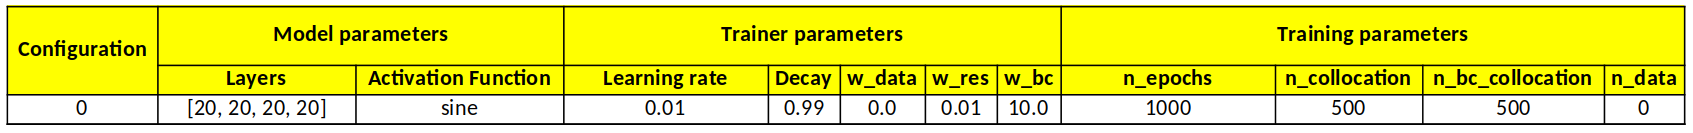
\includegraphics[width=0.8\linewidth]{"varier_f/config_0.png"}
	\caption{Paramètres du PINNs.}
	\label{config_0}
\end{figure}

On obtient les résultats d'entrainement suivant pour $S=0.55$ (car moyenne des paramètres) avec à gauche avec $f$ fixé et à droite avec $f$ qui varie :

\begin{minipage}{0.48\linewidth}
	\begin{figure}[H]
		\centering
		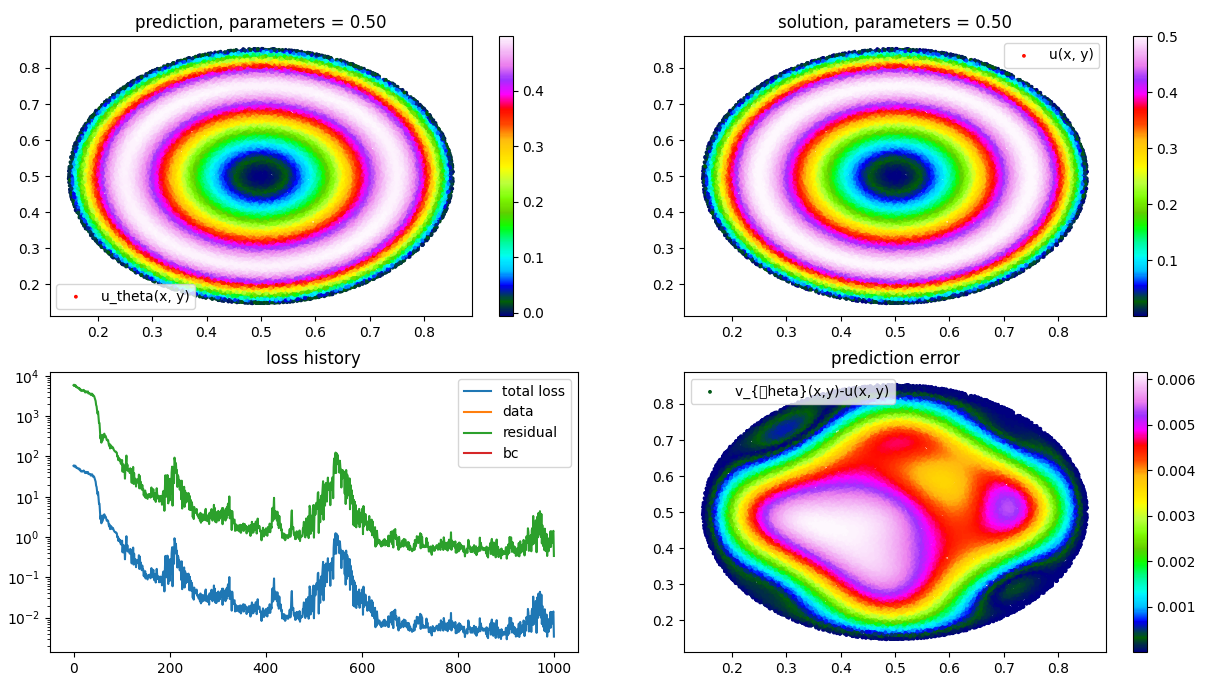
\includegraphics[width=0.9\linewidth]{"varier_f/Poisson2D_fixed_model_0_exact_bc.png"}
		\caption{Training $f$ fixé.}
		\label{Poisson2D_fixed_model_0_exact_bc}
	\end{figure}
\end{minipage}
\begin{minipage}{0.48\linewidth}
	\begin{figure}[H]
		\centering
		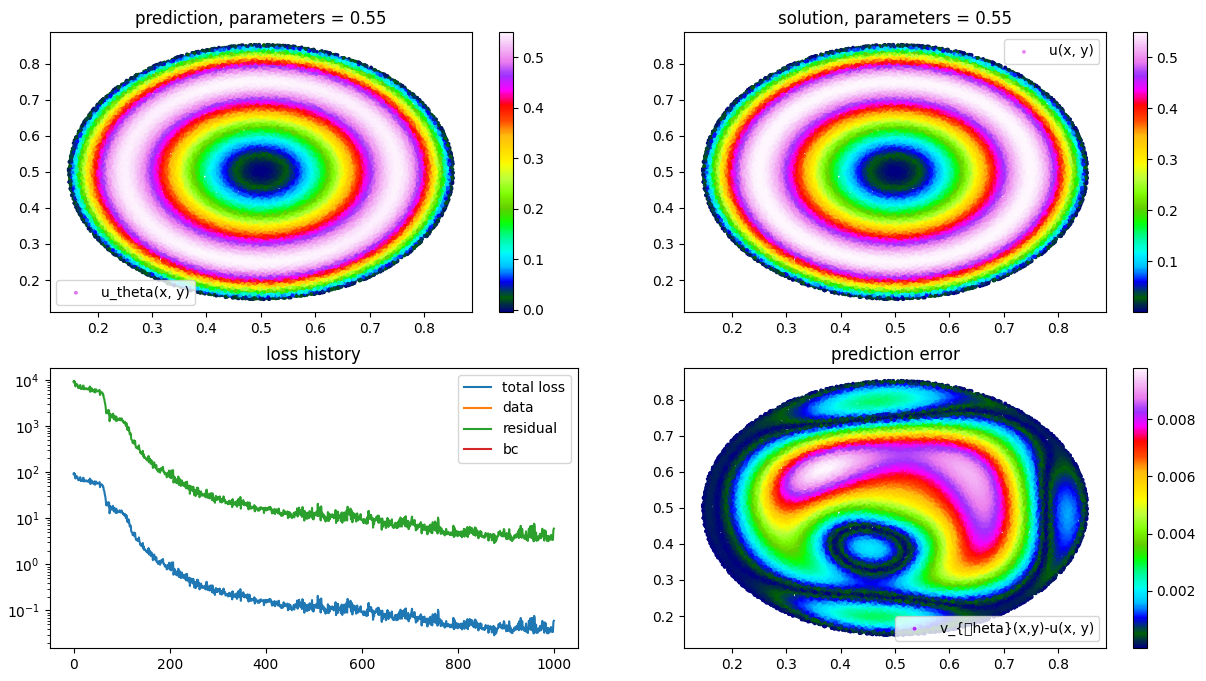
\includegraphics[width=0.9\linewidth]{"varier_f/Poisson2D_f_model_0_exact_bc.png"}
		\caption{Training $f$ qui varie.}
		\label{Poisson2D_f_model_0_exact_bc}
	\end{figure}
\end{minipage}

Pour $S=0.5$, on obtient les résultats suivants pour la correction par addition avec FEM :

\begin{minipage}{0.48\linewidth}
	\begin{figure}[H]
		\centering
		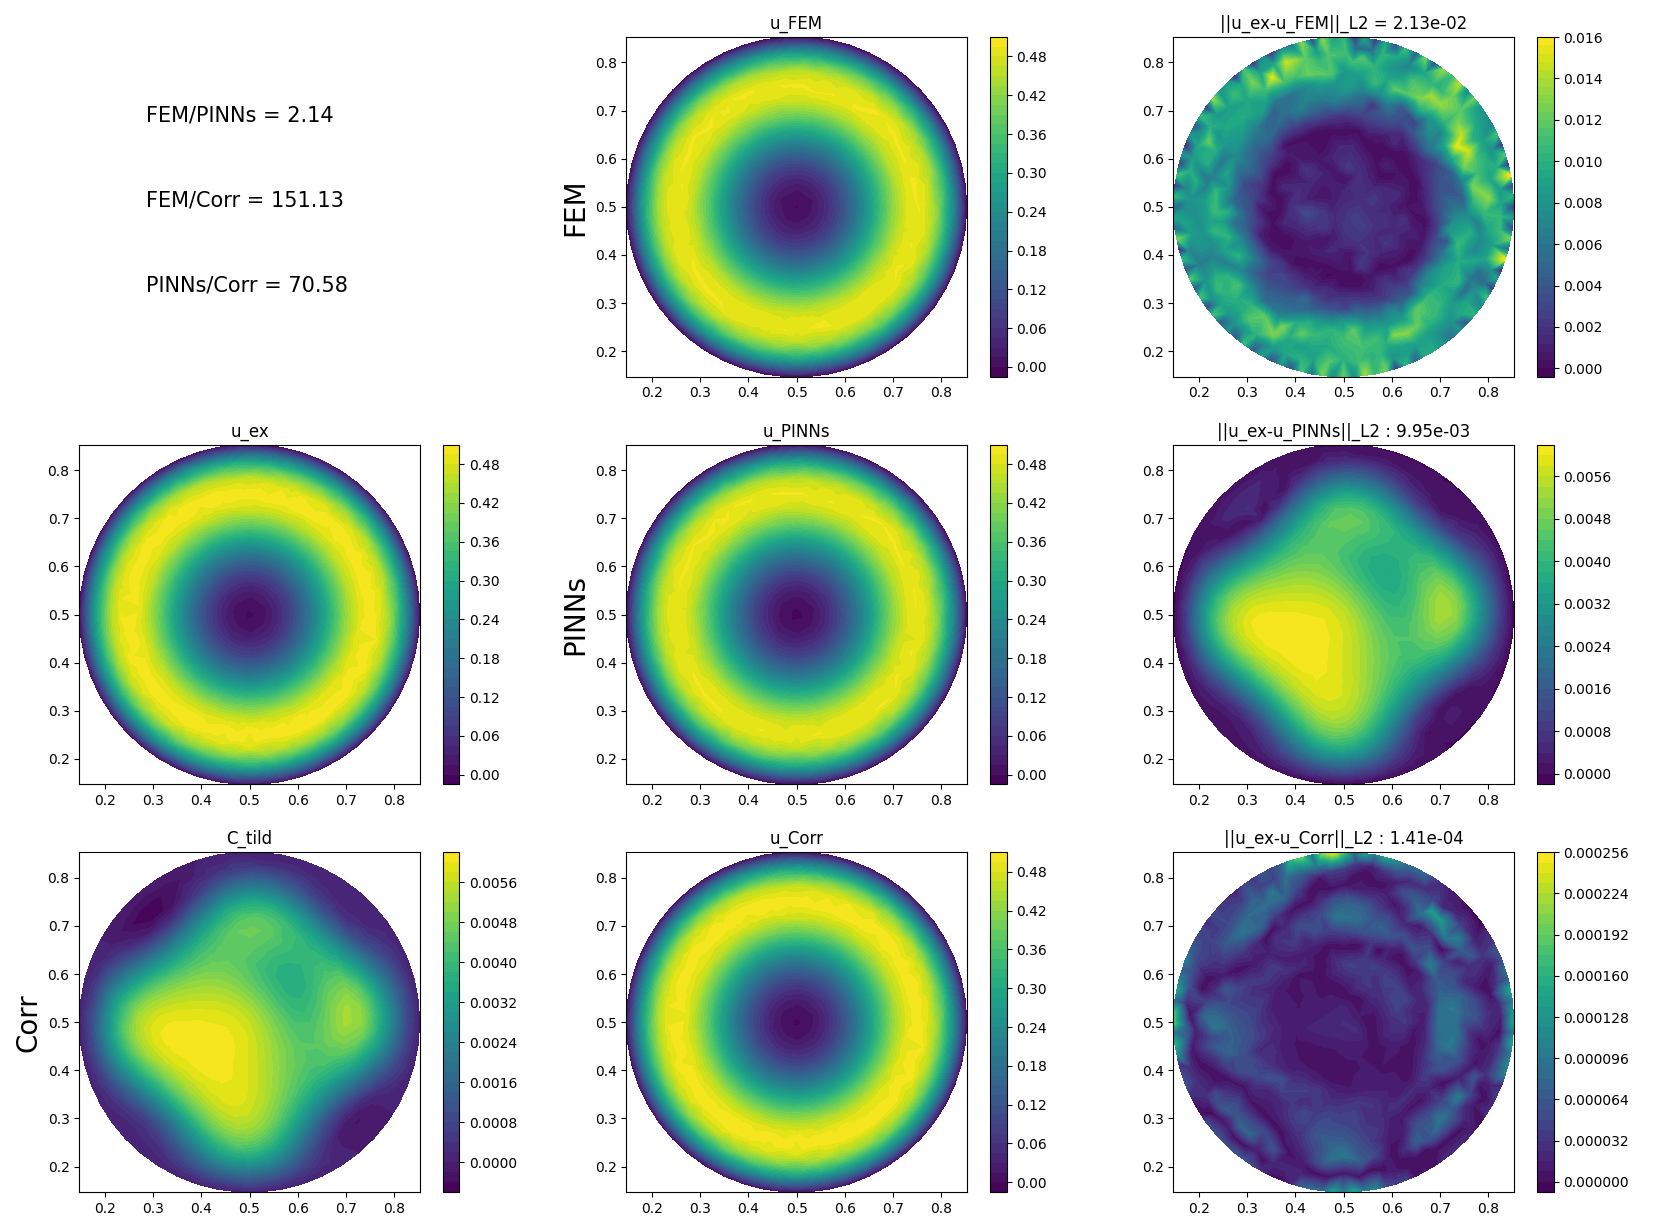
\includegraphics[width=0.88\linewidth]{"varier_f/Poisson2D_fixed_corr_fem_0_exact_bc.png"}
		\caption{Correction avec FEM - $f$ fixé.}
		\label{Poisson2D_fixed_corr_fem_0_exact_bc}
	\end{figure}
\end{minipage}
\begin{minipage}{0.48\linewidth}
	\begin{figure}[H]
		\centering
		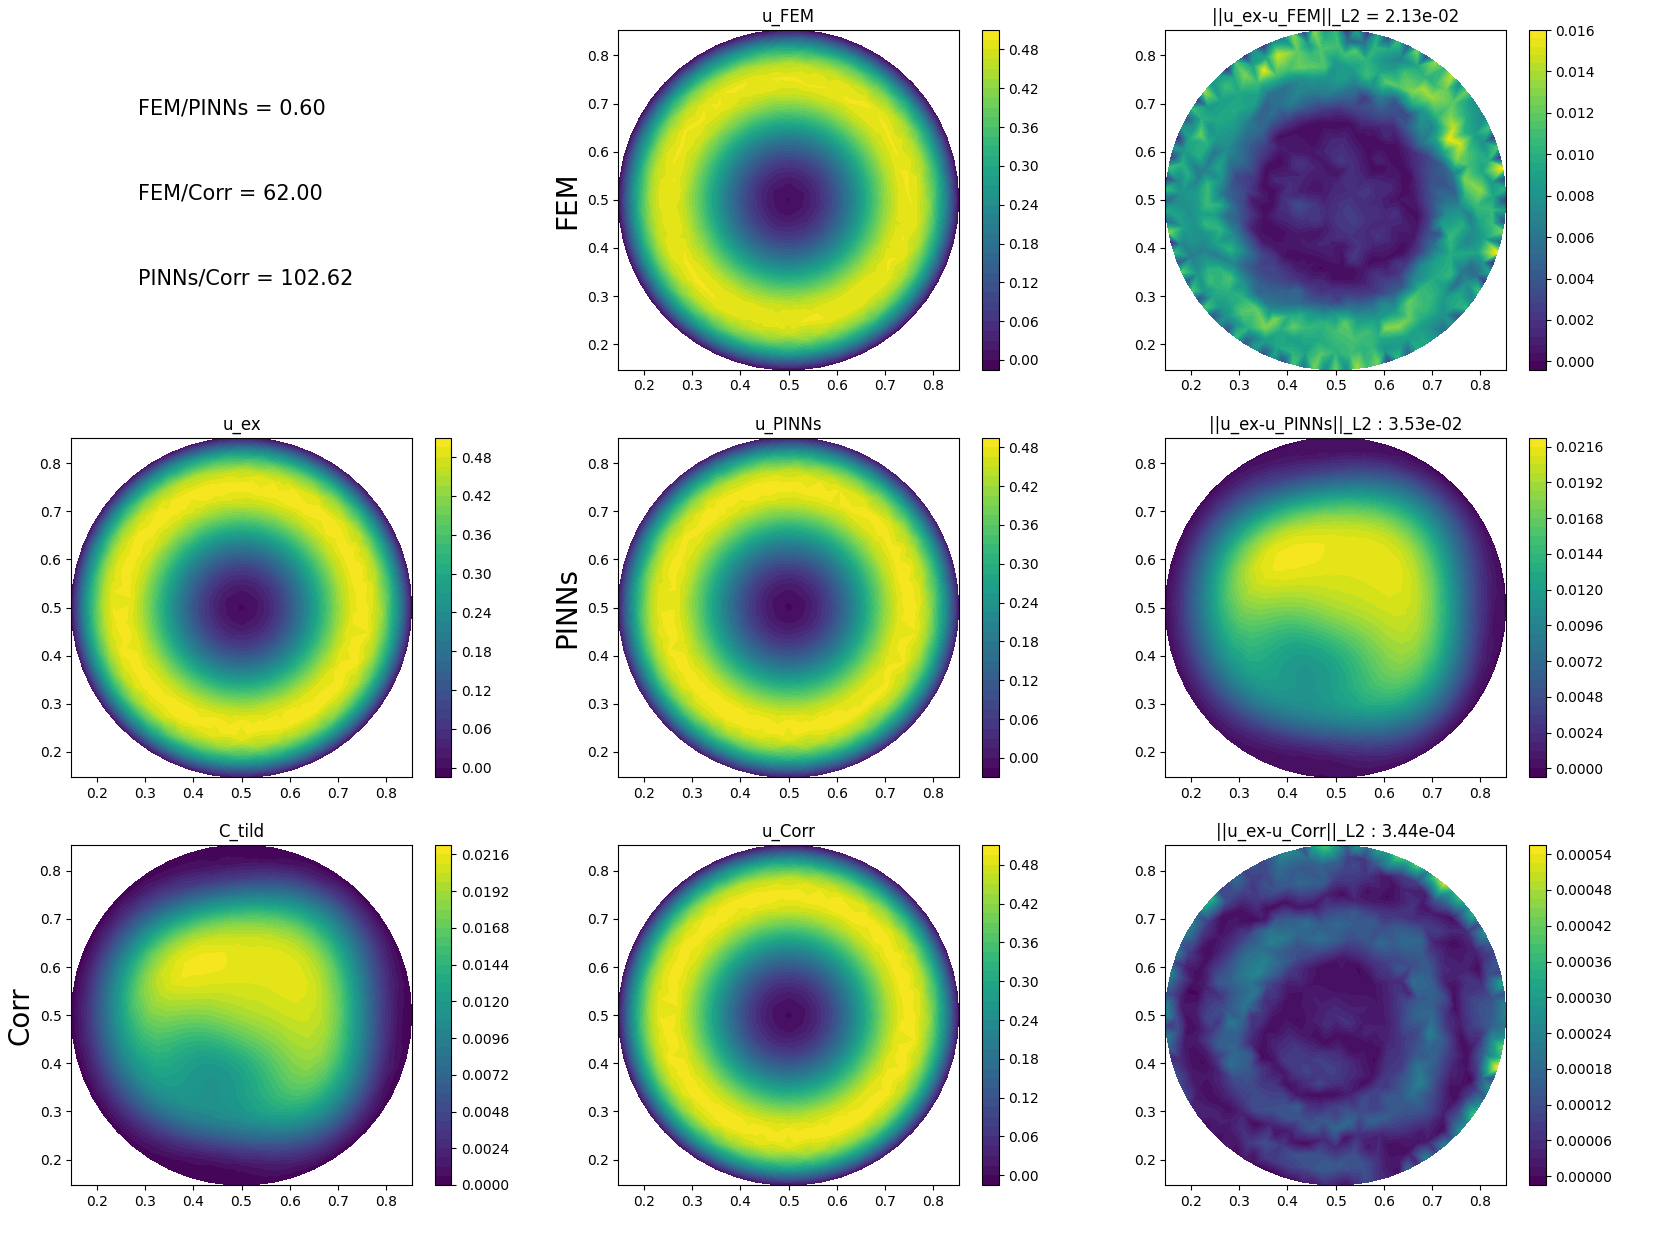
\includegraphics[width=0.88\linewidth]{"varier_f/Poisson2D_f_corr_fem_0_exact_bc.png"}
		\caption{Correction avec FEM - $f$ qui varie.}
		\label{Poisson2D_f_corr_fem_0_exact_bc}
	\end{figure}
\end{minipage}

Pour $S=0.5$, on obtient les résultats suivants pour la correction par addition avec $\phi$-FEM :

\begin{minipage}{0.48\linewidth}
	\begin{figure}[H]
		\centering
		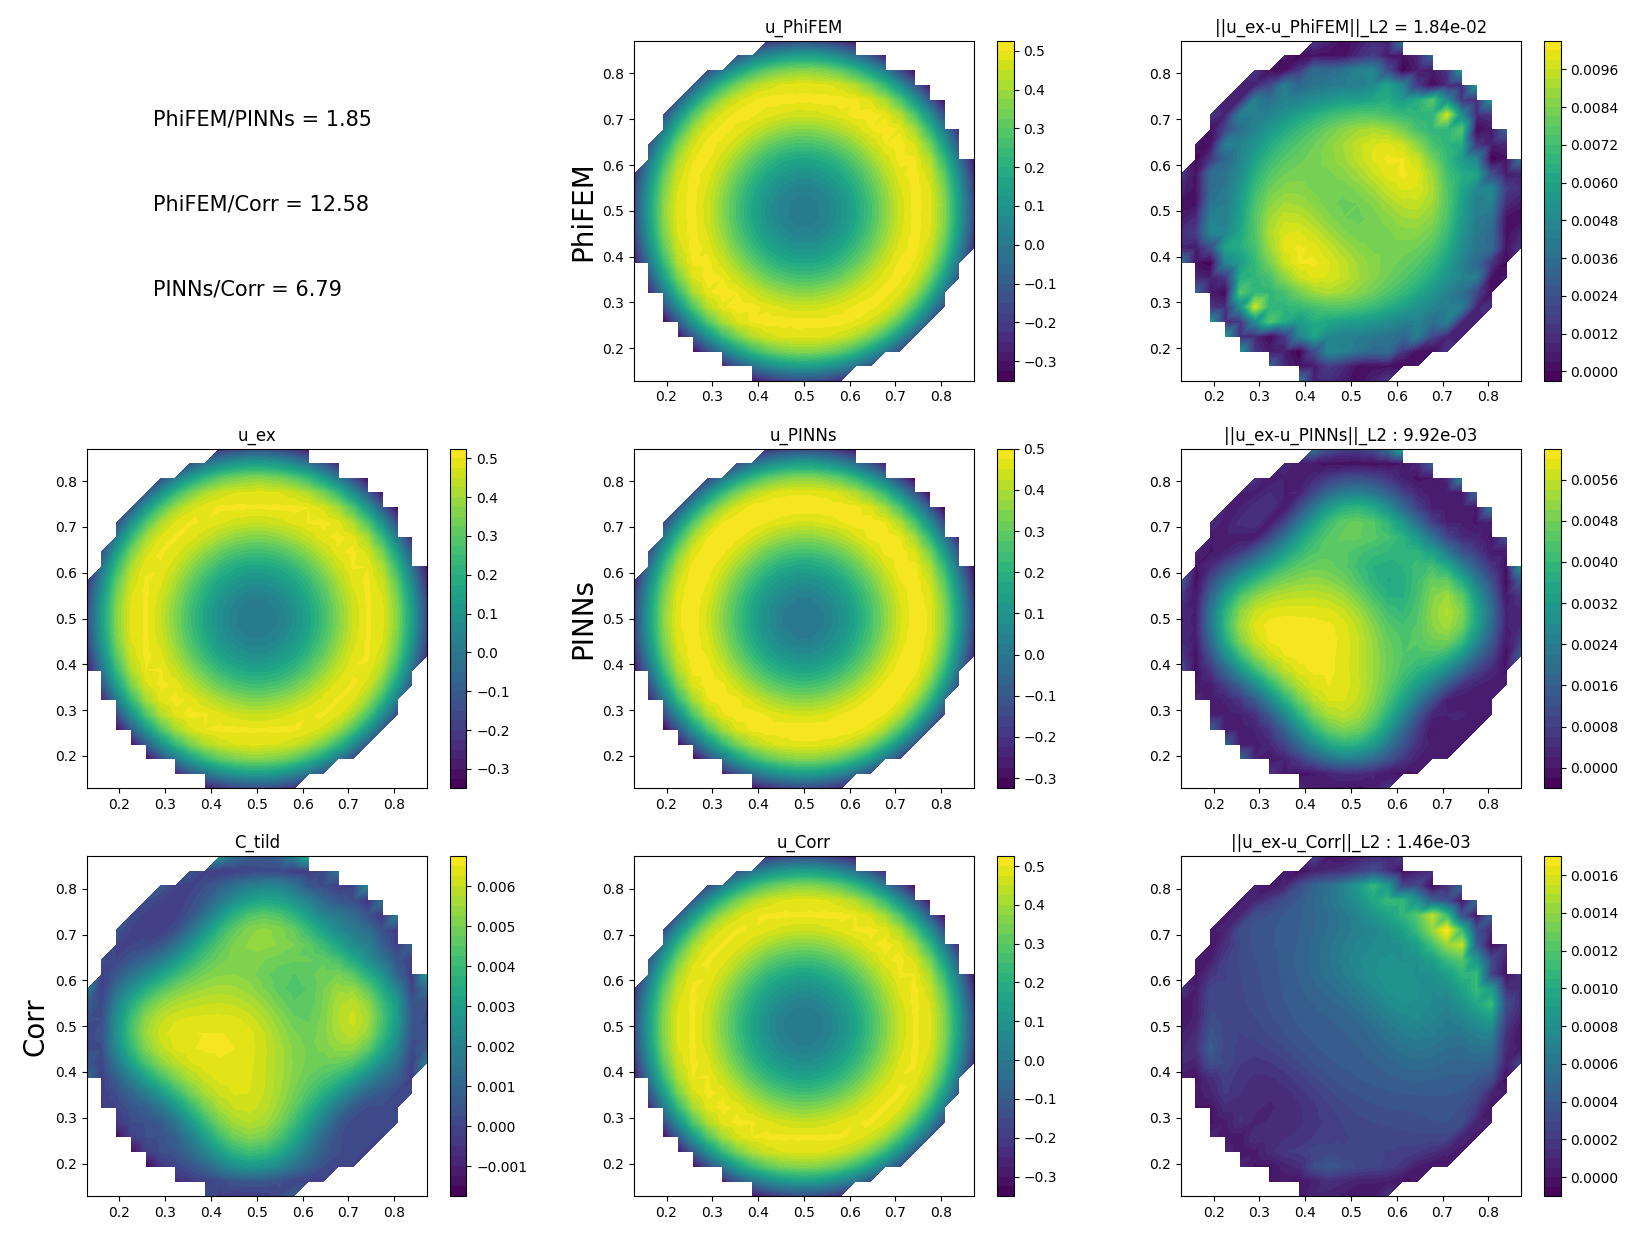
\includegraphics[width=0.88\linewidth]{"varier_f/Poisson2D_fixed_corr_phifem_0_exact_bc.png"}
		\caption{Correction avec $\phi$-FEM - $f$ fixé.}
		\label{Poisson2D_fixed_corr_phifem_0_exact_bc}
	\end{figure}
\end{minipage}
\begin{minipage}{0.48\linewidth}
	\begin{figure}[H]
		\centering
		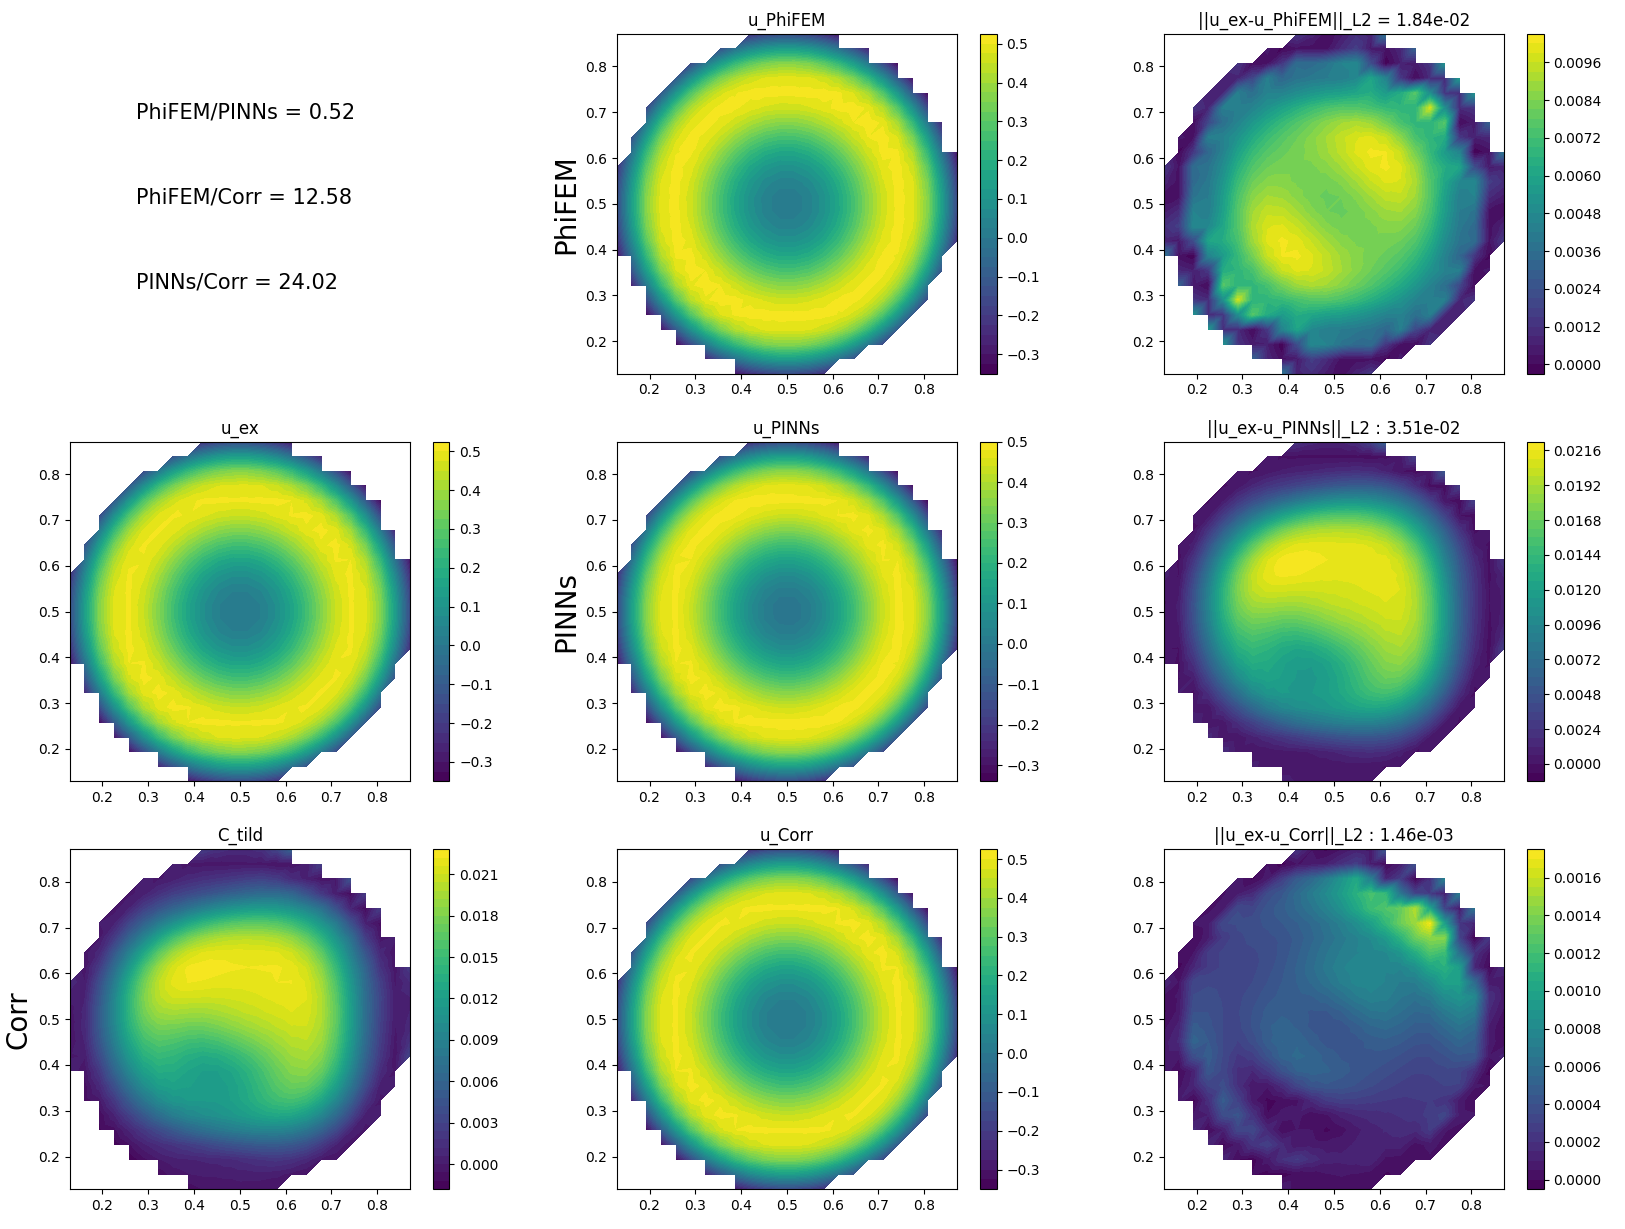
\includegraphics[width=0.88\linewidth]{"varier_f/Poisson2D_f_corr_phifem_0_exact_bc.png"}
		\caption{Correction avec $\phi$-FEM - $f$ qui varie.}
		\label{Poisson2D_f_corr_phifem_0_exact_bc}
	\end{figure}
\end{minipage}

\newpage

\section{Correction avec $\phi$-FEM sur la prédiction du modèle sur $w$ entraîné sur le carré}

On cherche ici à apprendre la même solution que précédemment mais on va entraîner le PINNs sur le carré tout entier (et pas seulement sur le cercle) dans le but de voir si la correction avec $\phi$-FEM est meilleure. On considère les même paramètres que dans le cas précédent mais avec plus de points (car sur le carré 500 n'tait pas suffisant) et entraîne le PINNs à déterminer $u=\phi w$ :

\begin{figure}[H]
	\centering
	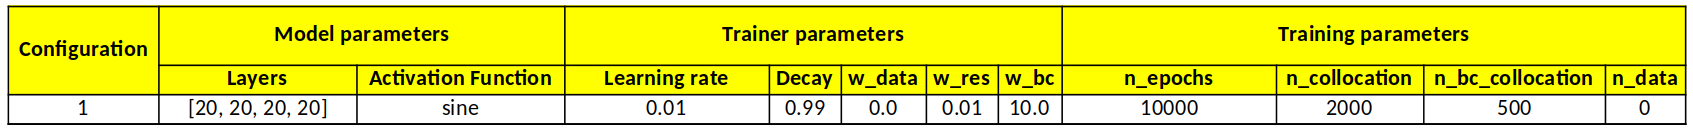
\includegraphics[width=\linewidth]{"train_sur_carre/Carre_config_1.png"}
	\caption{Paramètres du PINNs.}
	\label{config_1}
\end{figure}

\begin{minipage}{0.48\linewidth}
	\begin{figure}[H]
		\centering
		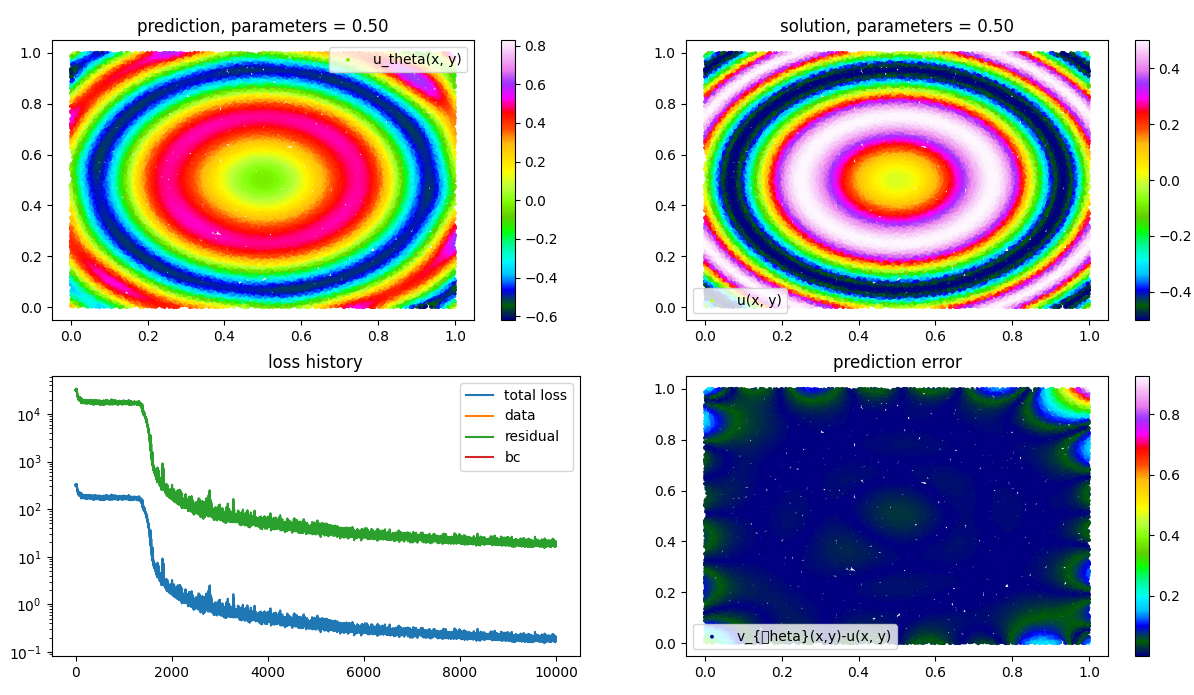
\includegraphics[width=\linewidth]{"train_sur_carre/Carre_model_1_exact_bc.png"}
		\caption{Training $f$ fixé sans le masque.}
		\label{Carre_model_1_exact_bc}
	\end{figure}
\end{minipage}
\begin{minipage}{0.48\linewidth}
	\begin{figure}[H]
		\centering
		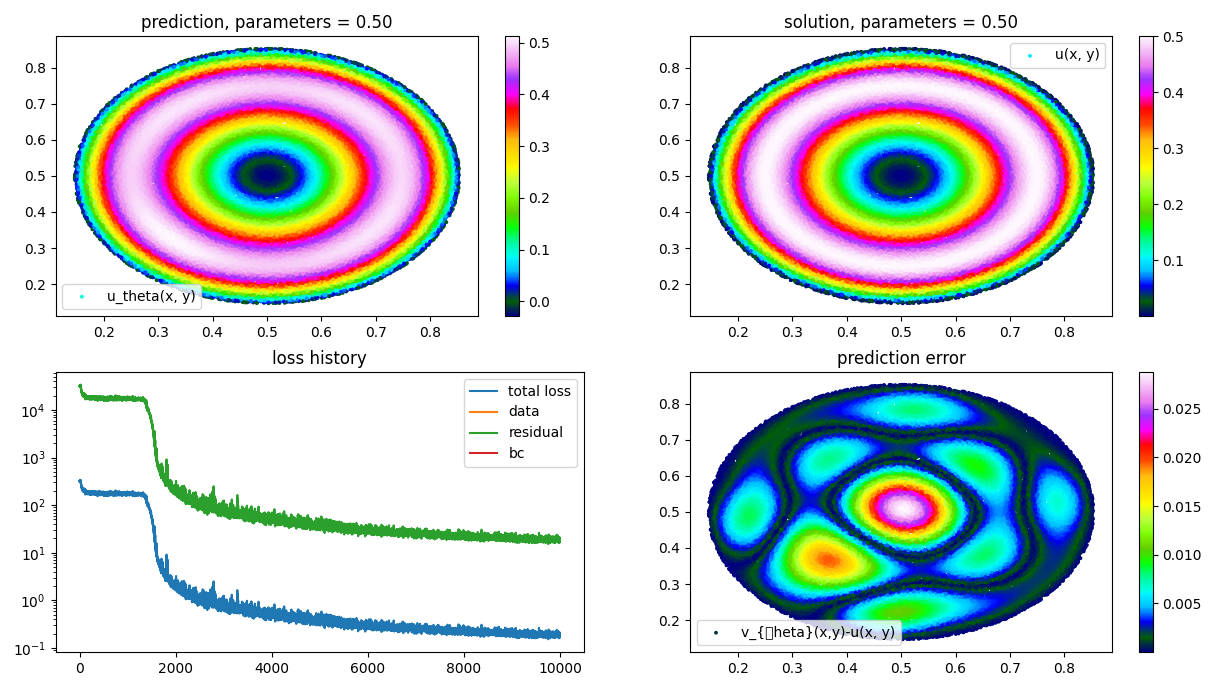
\includegraphics[width=\linewidth]{"train_sur_carre/Carre_model_1_exact_bc_mask.png"}
		\caption{Training $f$ fixé avec le masque.}
		\label{Carre_model_1_exact_bc_mask}
	\end{figure}
\end{minipage}

\begin{minipage}{0.48\linewidth}
	\begin{figure}[H]
		\centering
		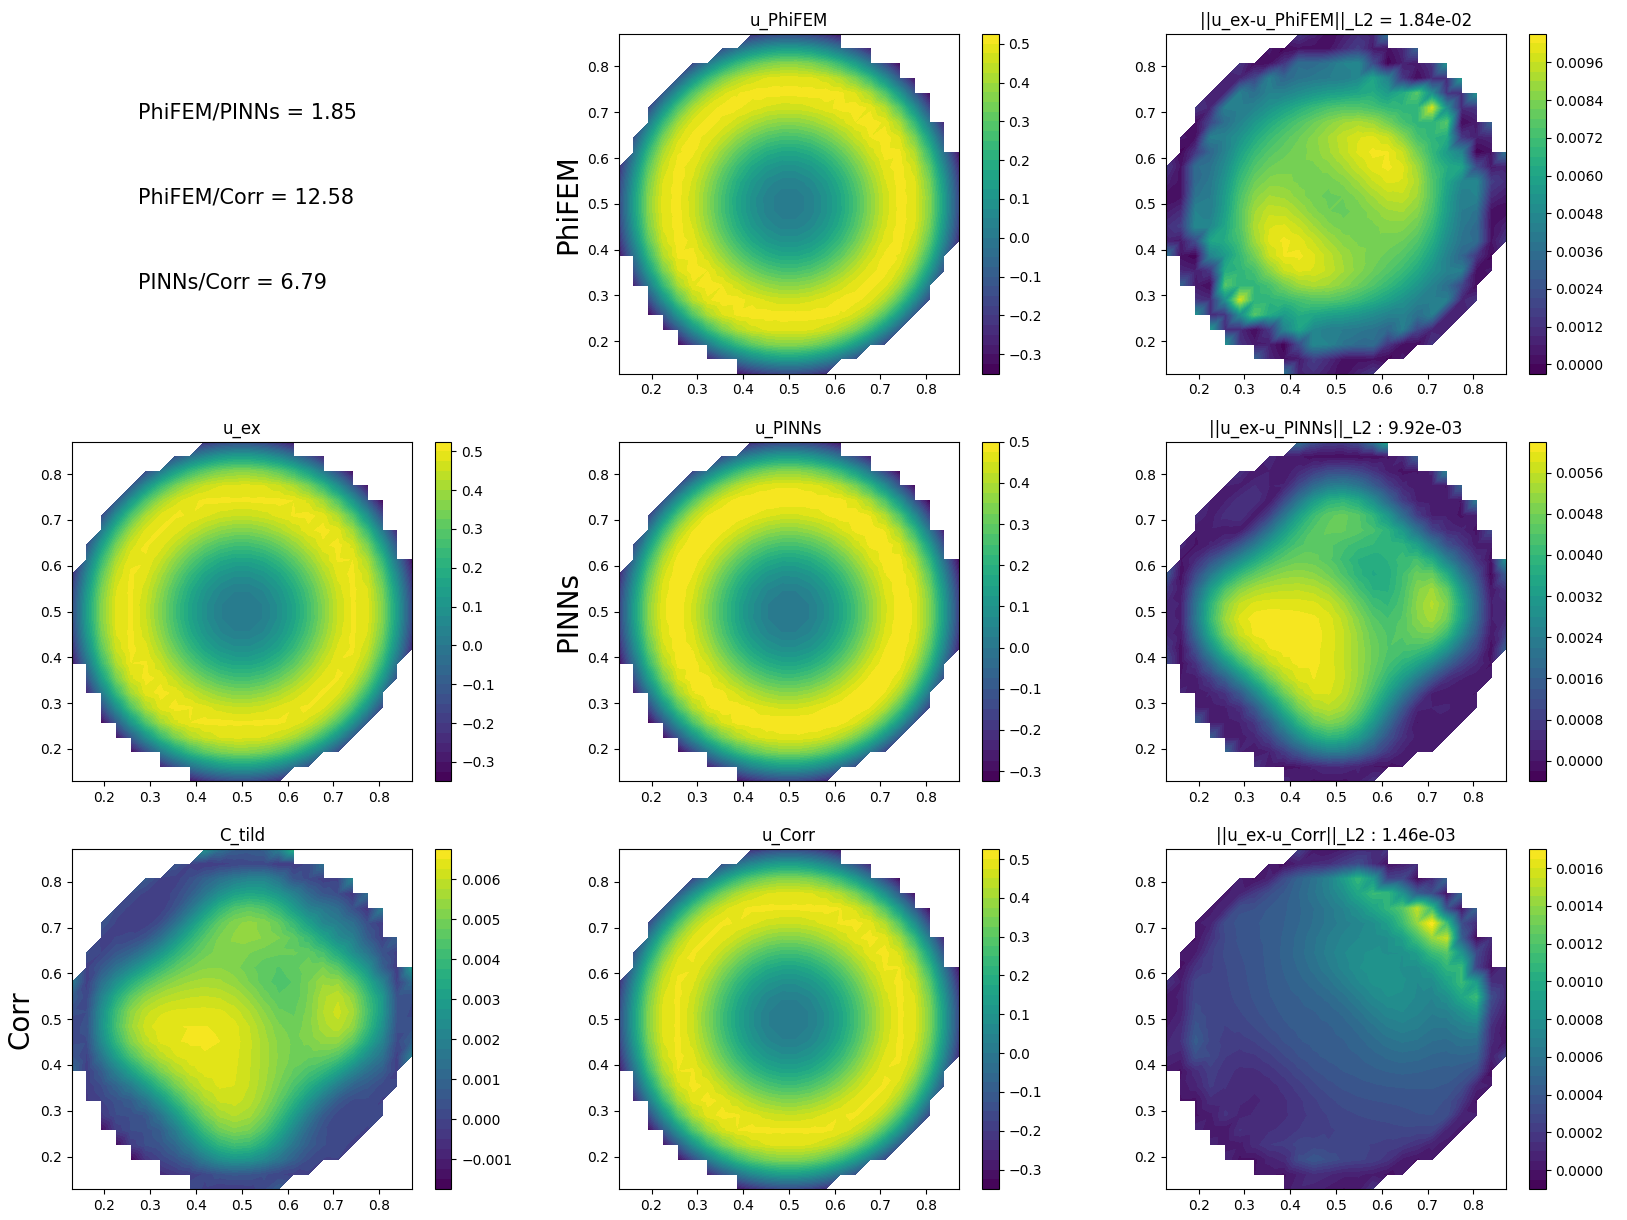
\includegraphics[width=\linewidth]{"train_sur_carre/Cercle_corr_phifem_0_exact_bc.png"}
		\caption{Correction avec $\phi$-FEM (en apprenant sur le cercle).}
		\label{Cercle_corr_phifem_0_exact_bc}
	\end{figure}
\end{minipage}
\begin{minipage}{0.48\linewidth}
	\begin{figure}[H]
		\centering
		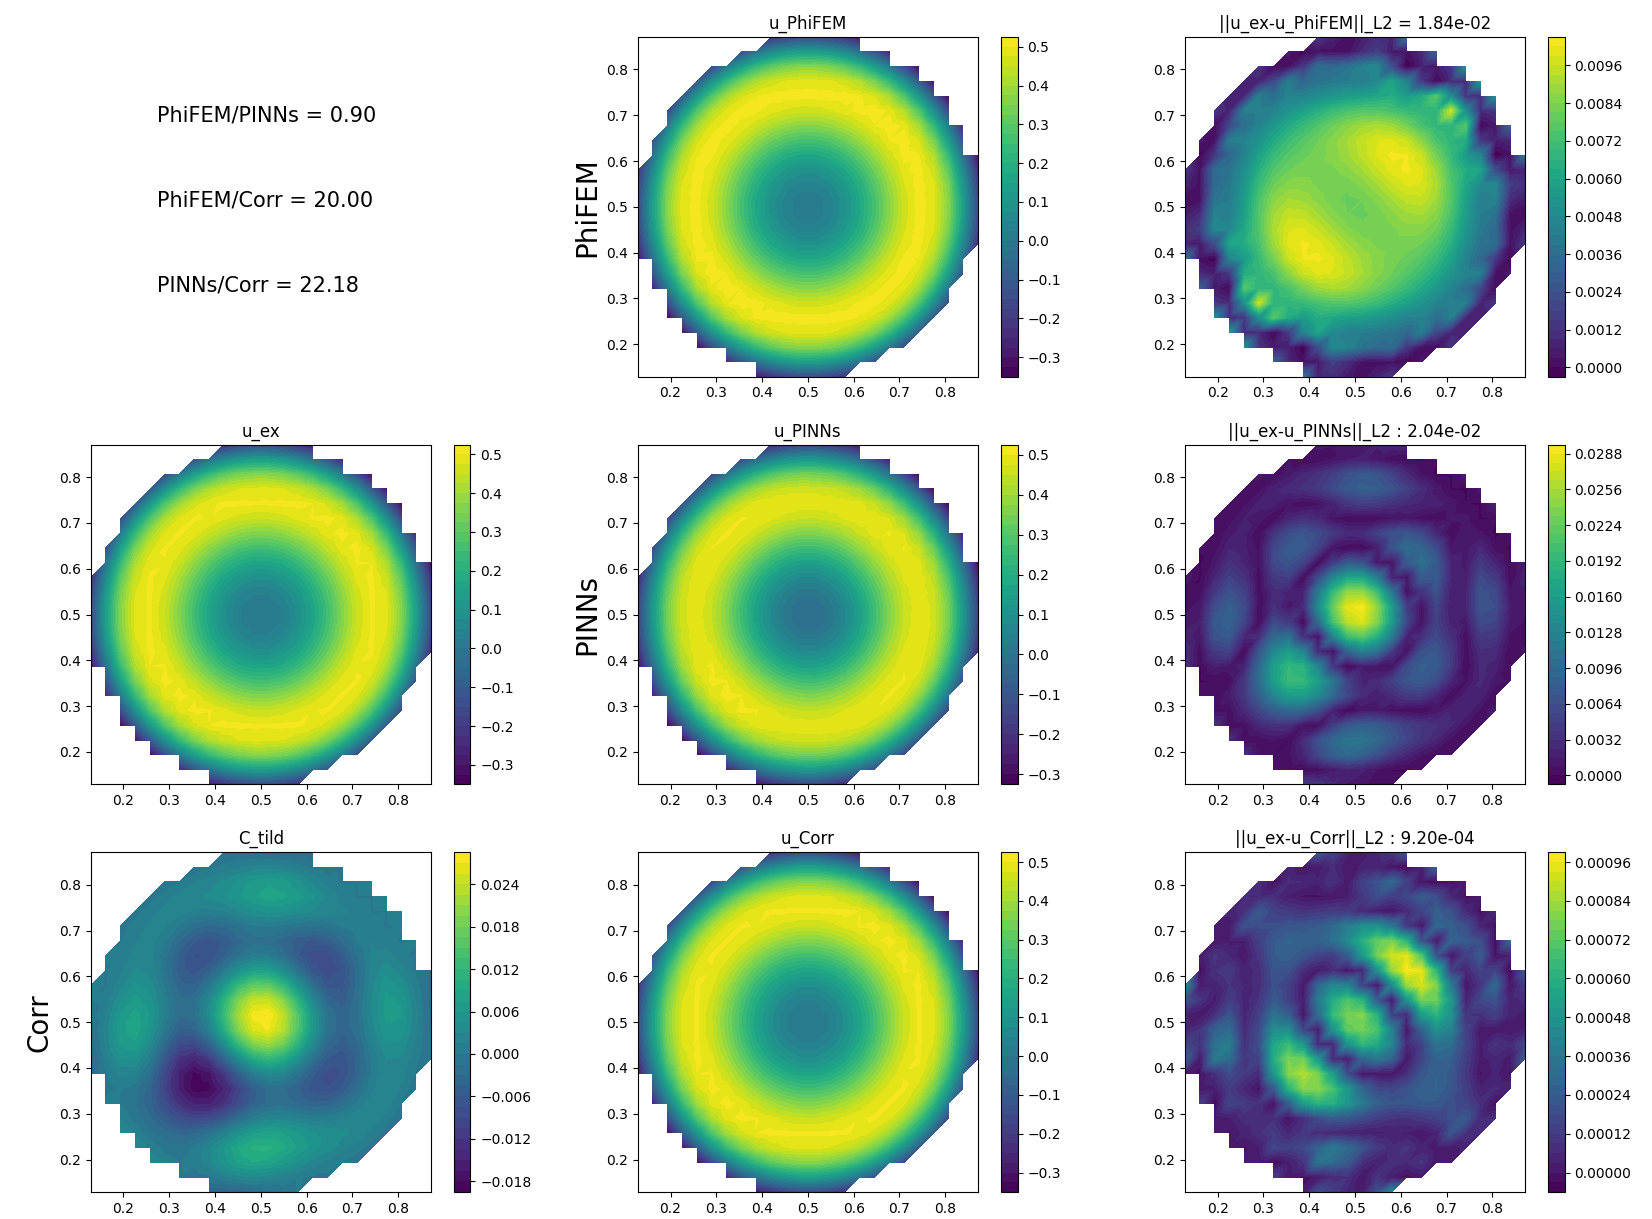
\includegraphics[width=\linewidth]{"train_sur_carre/Carre_corr_phifem_1_exact_bc.png"}
		\caption{Correction avec $\phi$-FEM (en apprenant sur le carré).}
		\label{Carre_corr_phifem_1_exact_bc}
	\end{figure}
\end{minipage}

\newpage

\section{Correction sur la prédiction du modèle sur $u$ avec recalage de la fonction levelset}

On fait une descente de gradient sur un certains nombres d'itérations dans le but de recaler la levelset sur le bord. A la fin la valeur de $\phi$ en les points choisis (en valeur absolu) est au maximum de 1e-17.

\begin{minipage}{0.48\linewidth}
	\begin{figure}[H]
		\centering
		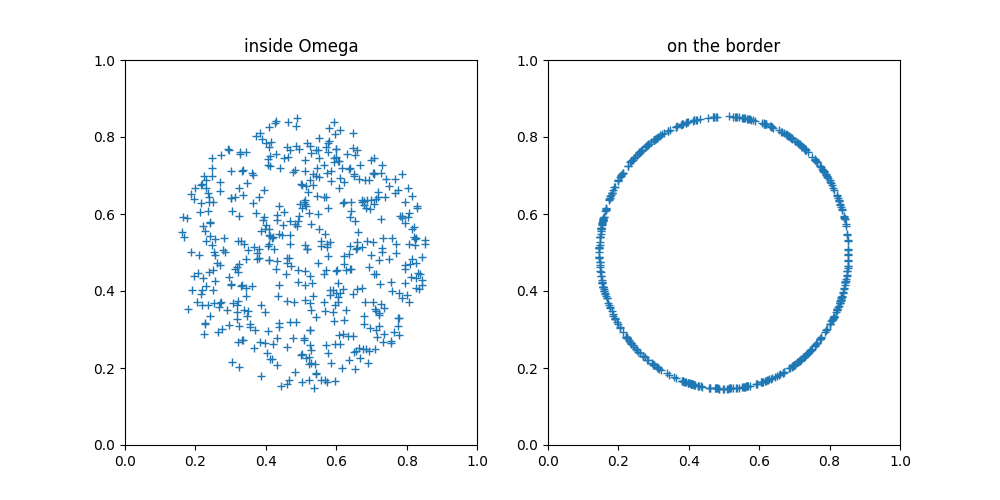
\includegraphics[width=\linewidth]{"recalage_levelset/sampling_0_align_levelset.png"}
		\caption{Sampling considéré.}
		\label{sampling_0_align_levelset}
	\end{figure}
\end{minipage}
\begin{minipage}{0.48\linewidth}
	\begin{figure}[H]
		\centering
		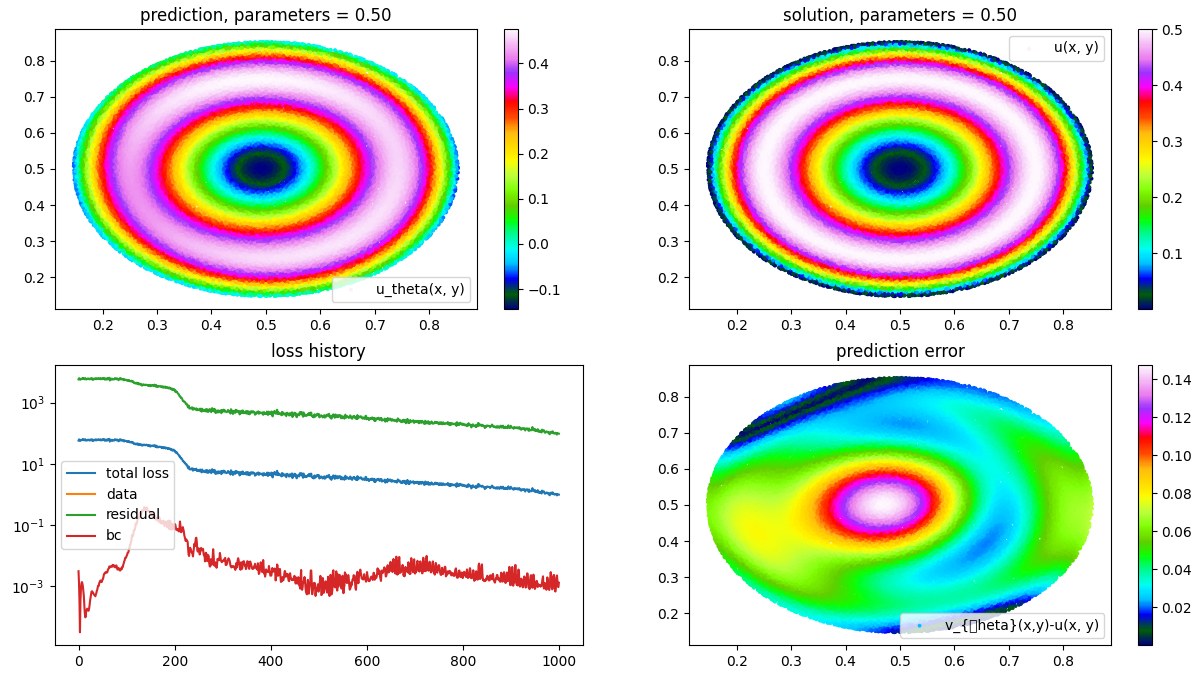
\includegraphics[width=\linewidth]{"recalage_levelset/model_0_align_levelset.png"}
		\caption{Entraînement avec recalage de la levelset.}
		\label{model_0_align_levelset}
	\end{figure}
\end{minipage}

On va essayer ici de modifier les paramètres et ré-entraîner le modèle de la manière suivante :

\begin{figure}[H]
	\centering
	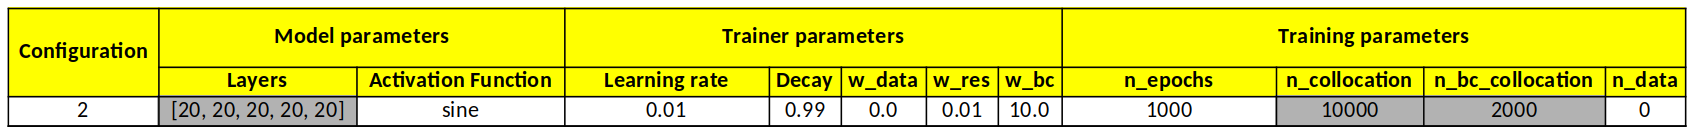
\includegraphics[width=\linewidth]{"recalage_levelset/config_align_levelset.png"}
	\caption{Paramètres du PINNs.}
	\label{config_align_levelset}
\end{figure}

\begin{minipage}{0.48\linewidth}
	\begin{figure}[H]
		\centering
		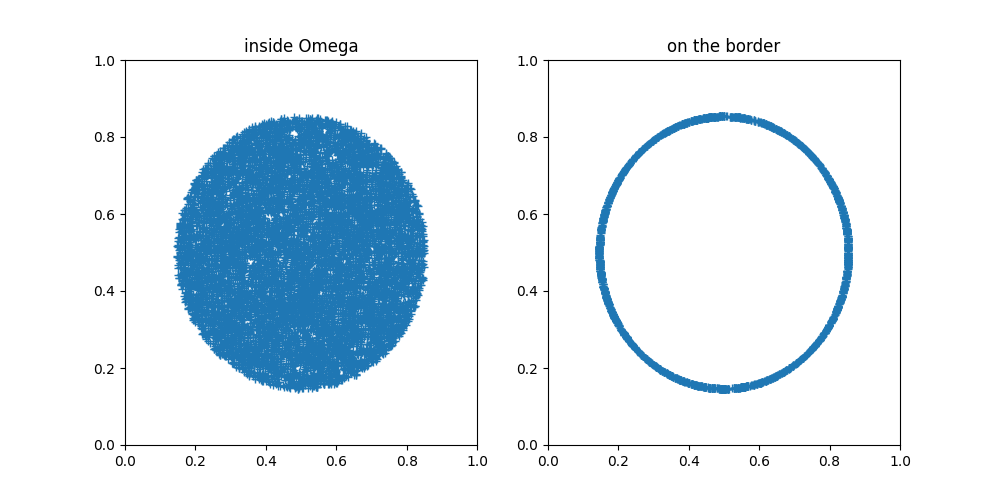
\includegraphics[width=\linewidth]{"recalage_levelset/sampling_2_align_levelset.png"}
		\caption{Sampling considéré.}
		\label{sampling_2_align_levelset}
	\end{figure}
\end{minipage}
\begin{minipage}{0.48\linewidth}
	\begin{figure}[H]
		\centering
		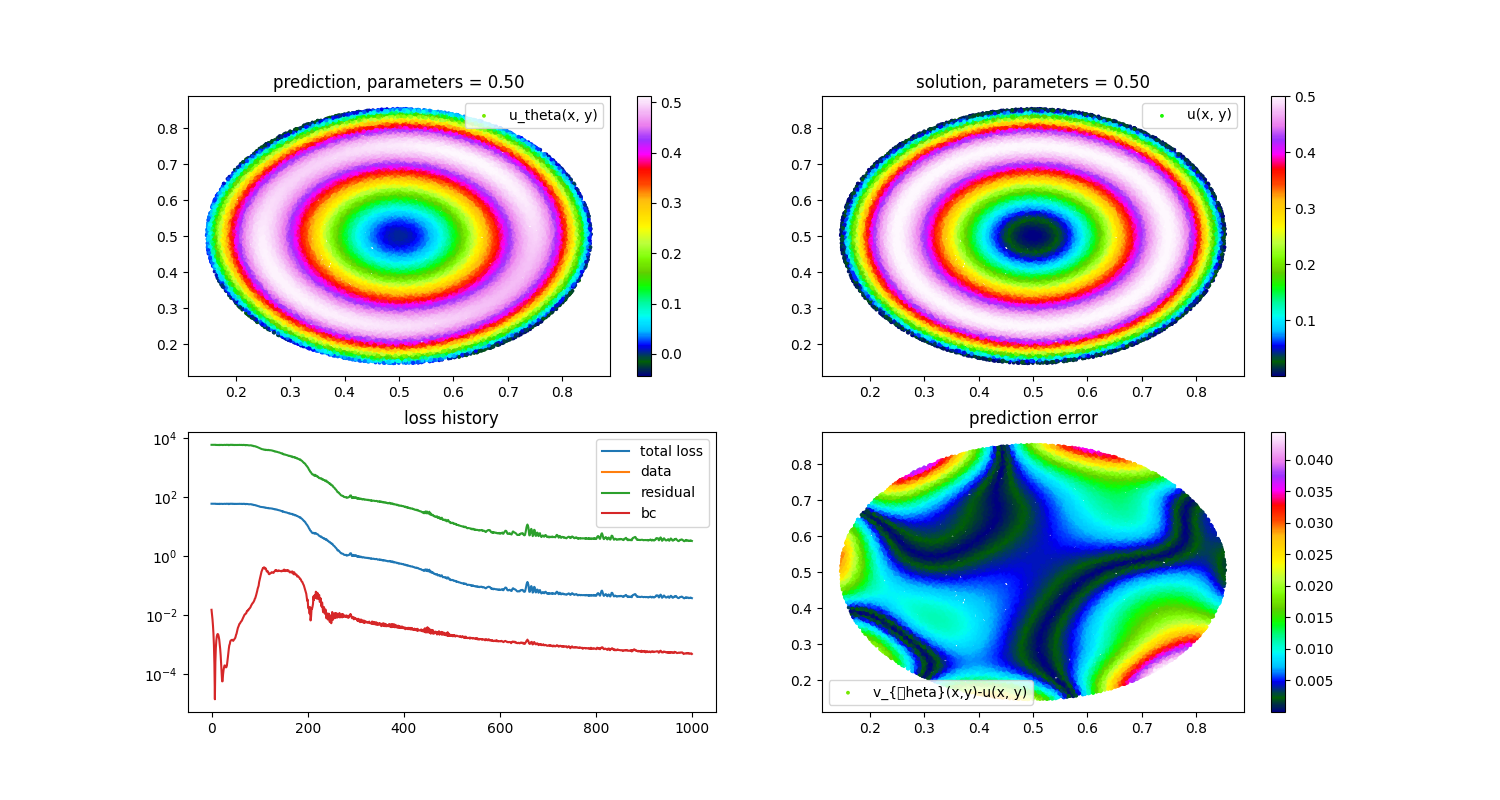
\includegraphics[width=\linewidth]{"recalage_levelset/model_2_align_levelset.png"}
		\caption{Entraînement avec recalage de la levelset.}
		\label{model_2_align_levelset}
	\end{figure}
\end{minipage}
